\documentclass[10pt]{article}
\usepackage[margin=0.6in]{geometry}
\usepackage[T1]{fontenc}
\usepackage{lmodern}
\usepackage{amsmath,amssymb}
\usepackage{booktabs,longtable,pdflscape,array,graphicx}
\makeatletter
\long\def\@makecaption#1#2{%
  \vskip\abovecaptionskip
  \sbox\@tempboxa{#2}%
  \ifdim \wd\@tempboxa >\hsize
    #2\par
  \else
    \global \@minipagefalse
    \hb@xt@\hsize{\hfil\box\@tempboxa\hfil}%
  \fi
  \vskip\belowcaptionskip}
\def\LT@makecaption#1#2#3{%
  \LT@mcol\LT@cols c{\hbox to\z@{\hss\parbox[t]\LTcapwidth{%
    \sbox\@tempboxa{#3}%
    \ifdim\wd\@tempboxa>\hsize
      #3%
    \else
      \hb@xt@\hsize{\hfil\box\@tempboxa\hfil}%
    \fi
    \endgraf\vskip\baselineskip}%
  \hss}}}
\makeatother
\setlength{\emergencystretch}{3em}
\sloppy
\graphicspath{{../results/graphs/}{../figures/}{./}}
\begin{document}
\section*{Supplementary Material: Case-Disjoint Benchmark of Surrogate Models for Flow and Thermal Fields in Supercritical CO$_2$ Natural-Circulation Loops}
This supplementary document provides:
\begin{itemize}
\item \textbf{Section S1 (Tables S0a--S0b):} Detailed loop geometry, pipe/wall/jacket radial dimensions, cross-sectional plane sampling counts (Table S0a), plane-weighted mean $\mathrm{CO}_2$ density summaries, and CoolProp $(\partial p/\partial T)_\rho$ values across operating subgroups (Table S0b).
\item \textbf{Figure S1:} Spatial field reconstructions and absolute error maps for the median (rank 21/42) and worst (rank 42/42) held-out cases by out-of-fold case-nMAE rank for density ($\rho$, \texttt{DeepONet}), temperature ($T$, \texttt{PINN continuity}), and vertical velocity ($v$, \texttt{Domain-informed FiLM-MLP}).
\item \textbf{Tables S1--S7:} Complete 20-row three-seed (\texttt{2026}, \texttt{2027}, \texttt{2028}) case-disjoint and within-group mesh-aligned field metrics across all 19 competing models plus the \texttt{Lattice floor (oracle)} voxel round-trip reconstruction reference for density ($\rho$), temperature ($T$), turbulence eddy dissipation ($\varepsilon$), turbulence kinetic energy ($k$), and velocity components ($u, v, w$).
\item \textbf{Table S8:} Complete 20-row three-seed gauge-pressure ($p_{\mathrm{gauge}}$) decomposition into case-level mean pressure error and centered spatial residual error (reporting both 42-case arithmetic-mean and 42-case root-mean-square residual RMSE).
\item \textbf{Table S9:} Complete three-seed leave-one-group-out shift metrics across the four structural/regime groups (\texttt{HHHC/small}, \texttt{HHVC/small}, \texttt{VHVC/small}, and \texttt{VHVC/large}; $16\text{ pooled models} \times 8\text{ fields} = 128$ model--field pairs per group).
\item \textbf{Table S10:} Exploratory nonparametric Friedman repeated-measures ranks, paired case-level median differences $\Delta$ with 95\% bootstrap confidence intervals, and within-field Holm-adjusted Wilcoxon signed-rank tests across the 42 cases.
\end{itemize}

\subsection*{S1. Detailed Conjugate Loop Geometry, Plane Sampling, and Thermodynamic Derivative Summary}
\begin{itemize}
\item \textbf{Small-scale loops (\texttt{HHHC}, 20 cases; \texttt{HHVC}, 5 cases; \texttt{VHVC}, 4 cases):} Centerline rectangular loop width $L_x = 0.8936\text{ m}$ ($x_{\mathrm{cl}} \in [0, 0.8936]\text{ m}$) and height $L_y = 1.0000\text{ m}$ ($y_{\mathrm{cl}} \in [0, 1.0000]\text{ m}$). The primary $\mathrm{sCO}_2$ fluid flows inside a circular pipe of inner diameter $D_i = 15.0\text{ mm}$ ($R_i = 7.50\text{ mm}$, $z \in [-7.50, +7.50]\text{ mm}$) surrounded by a $2.83\text{ mm}$ solid stainless-steel wall ($7.50 \le r \le 10.33\text{ mm}$, $\rho = 7969.4\text{ kg m}^{-3}$) and a $0.660\text{ m}$ concentric cooling-water jacket annulus ($10.33 \le r \le 12.96\text{ mm}$, outer jacket wall $12.96 \le r \le 15.65\text{ mm}$). In \texttt{HHHC}, the heater is on the bottom leg ($y_{\mathrm{cl}}=0$) and the cooler jacket spans $x \in [0.1168, 0.7768]\text{ m}$ on the top leg ($y_{\mathrm{cl}}=1.000\text{ m}$). In \texttt{HHVC} and small-loop \texttt{VHVC}, the cooler jacket is on the right vertical leg ($x_{\mathrm{cl}}=0.8936\text{ m}$), spanning $y \in [0.2232, 0.8832]\text{ m}$ and $y \in [0.2792, 0.9392]\text{ m}$, respectively, while the heater is on the bottom leg (\texttt{HHVC}) or lower left vertical leg (\texttt{VHVC}). Each small-loop case is exported on 97 cross-sectional planes (46 constant-$x$ and 51 constant-$y$ planes at $0.02\text{ m}$ nominal spacing), yielding $89,647\text{--}97,264$ primary $\mathrm{sCO}_2$ nodes per case ($\rho \le 950\text{ kg m}^{-3}$) after removing solid wall rows and $7,236\text{--}7,430$ outer cooling-water jacket nodes ($\rho \in [971.4, 1000.7]\text{ kg m}^{-3}$) and deduplicating intersecting plane coordinates.
\item \textbf{Large-scale loop (\texttt{VHVC}, 13 cases):} Centerline width $L_x = 3.0100\text{ m}$ ($x_{\mathrm{cl}} \in [0, 3.0100]\text{ m}$) and height $L_y = 4.0800\text{ m}$ ($y_{\mathrm{cl}} \in [0, 4.0800]\text{ m}$), with inner $\mathrm{sCO}_2$ pipe diameter $D_i = 13.84\text{ mm}$ ($R_i = 6.92\text{ mm}$, $z \in [-6.92, +6.92]\text{ mm}$), $3.58\text{ mm}$ solid stainless-steel wall ($6.92 \le r \le 10.50\text{ mm}$, $\rho = 7971.8\text{ kg m}^{-3}$), and a $1.130\text{ m}$ vertical cooler jacket on the right leg ($x_{\mathrm{cl}}=3.0100\text{ m}$, $y \in [2.220, 3.350]\text{ m}$, cooling-water annulus $10.50 \le r \le 38.93\text{ mm}$, outer jacket wall $38.93 \le r \le 45.80\text{ mm}$). Each large-loop case is sampled on 142 unique cross-sectional planes (61 constant-$x$ and 81 constant-$y$ planes at $0.05\text{ m}$ nominal spacing; raw exports contain 284 plane blocks due to a duplicated plane pass removed during coordinate deduplication), yielding $207,586$ primary $\mathrm{sCO}_2$ nodes per case (and $82,185$ outer cooling-water jacket nodes).
\end{itemize}

\begin{table}[htbp]
\centering
\scriptsize
\caption{Table S0a: Structural loop dimensions, radial conjugate layers, and cross-sectional sampling plane counts across the four configuration/scale groups.}
\resizebox{\textwidth}{!}{%
\begin{tabular}{llrrrrrrr}
\toprule
Group & Cases & $L_x \times L_y$ (m) & $D_i$ (mm) & Wall $r$ (mm) & Jacket $r$ (mm) & Unique planes & Primary $\mathrm{sCO}_2$ nodes/case & Water jacket nodes/case \\
\midrule
\texttt{HHHC/small} & 20 & $0.8936 \times 1.0000$ & 15.00 & 7.50--10.33 & 10.33--12.96 & 97 (46$x$+51$y$) & 97,264 & 7,430 \\
\texttt{HHVC/small} & 5  & $0.8936 \times 1.0000$ & 15.00 & 7.50--10.33 & 10.33--12.96 & 97 (46$x$+51$y$) & 89,771 & 7,236 \\
\texttt{VHVC/small} & 4  & $0.8936 \times 1.0000$ & 15.00 & 7.50--10.33 & 10.33--12.96 & 97 (46$x$+51$y$) & 89,647 & 7,236 \\
\texttt{VHVC/large} & 13 & $3.0100 \times 4.0800$ & 13.84 & 6.92--10.50 & 10.50--38.93 & 142 (61$x$+81$y$) & 207,586 & 82,185 \\
\bottomrule
\end{tabular}%
}
\end{table}

\begin{table}[htbp]
\centering
\scriptsize
\caption{Table S0b: Summary of plane-weighted mean $\mathrm{CO}_2$ density $\bar{\rho}_{\mathrm{plane},c}$, loop-mean temperature $\bar{T}_c$, case-mean gauge pressure $\bar{p}_c$, and CoolProp $(\partial p/\partial T)_\rho$ evaluated at $(\bar{\rho}_{\mathrm{plane},c}, \bar{T}_c)$ across operating subgroups.}
\resizebox{\textwidth}{!}{%
\begin{tabular}{llrrrrrrr}
\toprule
Group & $(p_{\mathrm{op}}, T_{\mathrm{in}})$ & Cases & Planes & $\bar{\rho}_{\mathrm{plane},c}$ (kg m$^{-3}$) & $\mathrm{SD}(\bar{\rho}_{\mathrm{plane},c})$ & $\bar{T}_c$ ($^\circ$C) & $\bar{p}_c$ (MPa) & CoolProp $(\partial p/\partial T)_\rho$ (MPa K$^{-1}$) \\
\midrule
\texttt{HHHC/small} & 80 bar, 305 K & 3 & 97 & 582.0--612.5 & 16.06 & 34.43--35.85 & 0.360--0.464 & 0.235--0.255 \\
\texttt{HHHC/small} & 90 bar, 300 K & 3 & 97 & 737.7--756.1 & 9.23  & 30.89--33.24 & 0.281--0.553 & 0.393--0.417 \\
\texttt{HHHC/small} & 90 bar, 305 K & 8 & 97 & 671.6--704.0 & 9.79  & 33.42--36.14 & 0.223--0.504 & 0.315--0.349 \\
\texttt{HHHC/small} & 90 bar, 315 K & 3 & 97 & 376.2--389.4 & 6.62  & 45.28--47.52 & 0.365--0.520 & 0.133--0.139 \\
\texttt{HHHC/small} & 100 bar, 305 K & 3 & 97 & 709.1--723.2 & 7.09 & 35.12--37.38 & 0.319--0.631 & 0.362--0.377 \\
\texttt{HHVC/small} & 90 bar, 305 K & 5 & 97 & 681.2--717.8 & 16.66 & 31.92--39.36 & 0.006--1.763 & 0.332--0.365 \\
\texttt{VHVC/small} & 90 bar, 305 K & 4 & 97 & 696.8--712.1 & 6.62  & 32.63--34.59 & 0.131--0.513 & 0.342--0.358 \\
\texttt{VHVC/large} & 85 bar, 283.5 K & 13 & 142 & 161.5--860.8 & 270.83 & 16.48--92.22 & 0.001--0.009 & 0.039--0.596 \\
\bottomrule
\end{tabular}%
}
\end{table}

\newpage
\begin{figure}[htbp]
\centering
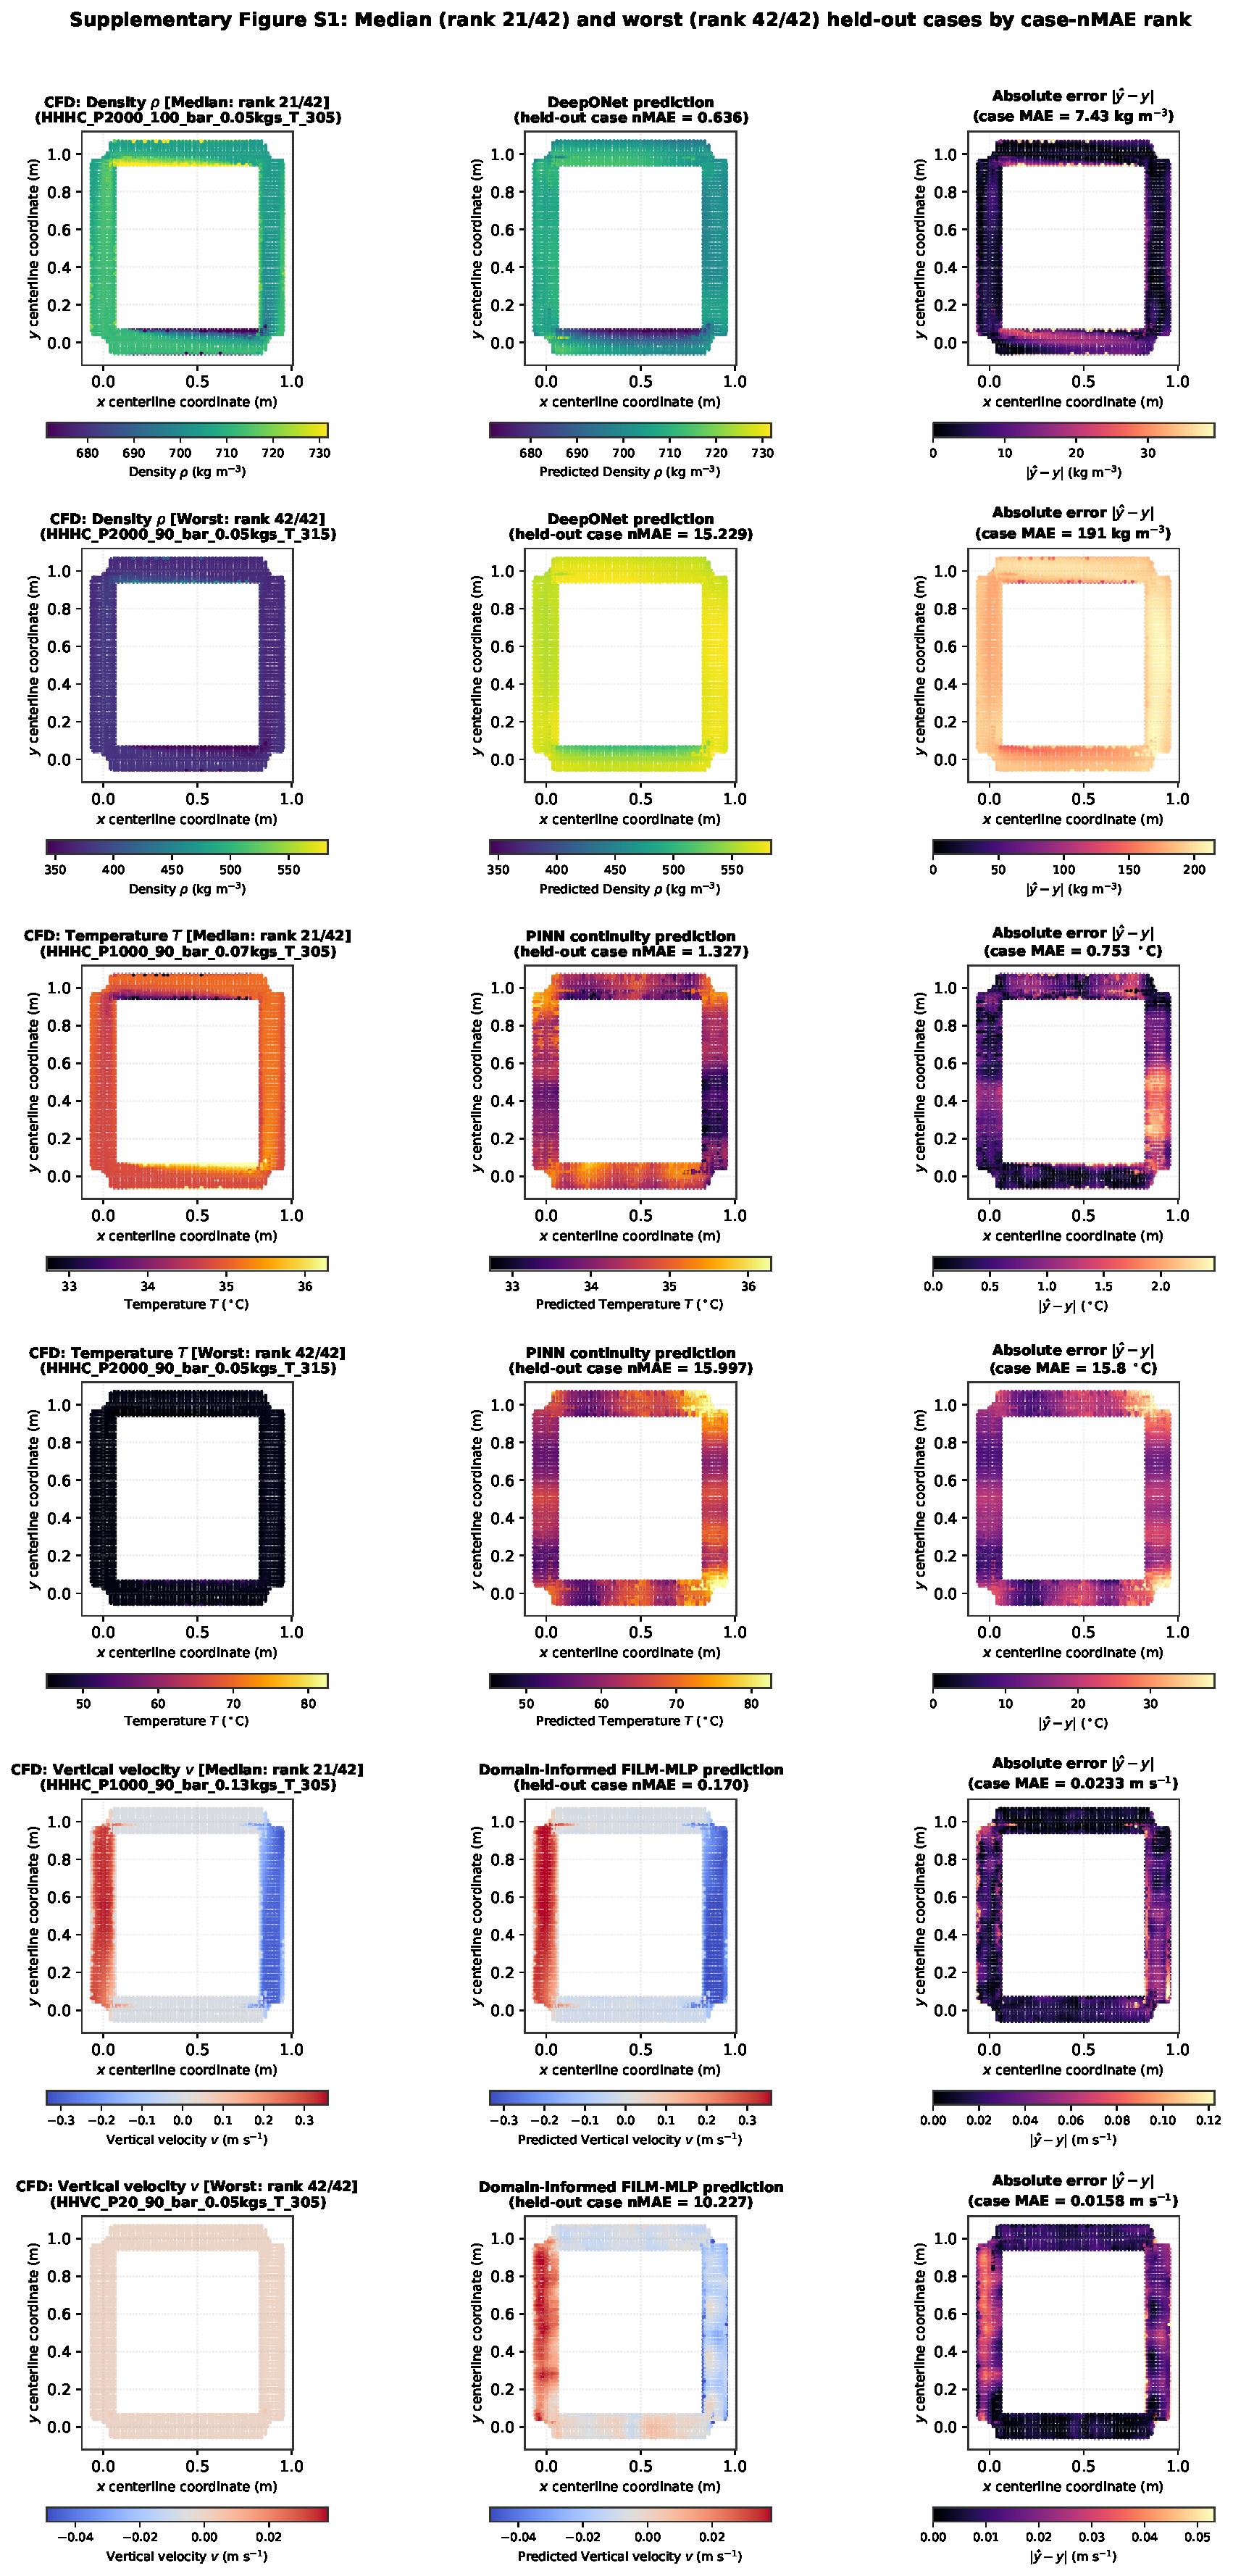
\includegraphics[width=0.92\textwidth,height=0.90\textheight,keepaspectratio]{heldout_cfd_prediction_error_maps_median_worst.pdf}
\caption{Figure S1: Out-of-fold spatial reconstructions and absolute error maps for the median (rank 21/42) and worst (rank 42/42) held-out cases selected by case-nMAE rank (seed 2026) for density $\rho$ (\texttt{DeepONet}), temperature $T$ (\texttt{PINN continuity}), and vertical velocity $v$ (\texttt{Domain-informed FiLM-MLP}).}
\end{figure}
\clearpage

\begin{landscape}\scriptsize
\begin{longtable}{p{3.8cm}p{2.9cm}rrrrrr}
\caption{Table S1: Complete three-seed (2026, 2027, 2028) out-of-fold benchmark metrics for Density ($\rho$, kg m$^{-3}$) across all 42 primary $\mathrm{sCO}_2$ cases. Entries report three-seed mean $\pm$ SD of median case nMAE, mean interquartile range (IQR), mean 95\% case-bootstrap CI, case-macro MAE, case-macro RMSE, and pooled $R^2$.}\\
\toprule Model & Protocol & Median nMAE ($\pm$SD) & nMAE IQR & 95\% Bootstrap CI & Macro MAE & Macro RMSE & Pooled $R^2$\\
\midrule\endfirsthead
\toprule Model & Protocol & Median nMAE ($\pm$SD) & nMAE IQR & 95\% Bootstrap CI & Macro MAE & Macro RMSE & Pooled $R^2$\\
\midrule\endhead
DeepONet & Case-disjoint 5-fold & 0.837 $\pm$ 0.16 & [0.473, 2.24] & [0.611, 1.71] & 35.1 & 37.1 & 0.862 \\
POD-RBF & Within-group aligned & 0.966 $\pm$ 0.28 & [0.295, 2.06] & [0.543, 1.46] & 34.4 & 35.2 & 0.883 \\
Domain-informed Concat-MLP & Case-disjoint 5-fold & 1.01 $\pm$ 0.069 & [0.583, 2.3] & [0.719, 1.5] & 26.3 & 29.1 & 0.936 \\
Domain-informed FiLM-MLP & Case-disjoint 5-fold & 1.04 $\pm$ 0.26 & [0.447, 2.49] & [0.632, 1.7] & 31.3 & 33.2 & 0.913 \\
PINN data-only & Case-disjoint 5-fold & 1.16 $\pm$ 0.098 & [0.617, 2] & [0.858, 1.43] & 30.6 & 33.8 & 0.914 \\
PINN continuity & Case-disjoint 5-fold & 1.17 $\pm$ 0.021 & [0.658, 2.4] & [0.85, 1.65] & 33.6 & 36.6 & 0.901 \\
Nearest case & Within-group aligned & 1.18 $\pm$ 0.15 & [0.633, 2.47] & [0.849, 1.76] & 45.1 & 46.5 & 0.792 \\
GAMS-GNN-style & Case-disjoint 5-fold & 1.25 $\pm$ 0.14 & [0.752, 2.01] & [0.88, 1.65] & 31.8 & 34.8 & 0.917 \\
Transolver-style & Case-disjoint 5-fold & 1.28 $\pm$ 0.22 & [0.705, 2.14] & [0.869, 1.58] & 32.9 & 35.6 & 0.903 \\
Latent Neural Operator & Case-disjoint 5-fold & 1.32 $\pm$ 0.18 & [0.651, 2.66] & [0.904, 1.92] & 34.1 & 37.8 & 0.882 \\
XGBoost & Case-disjoint 5-fold & 1.42 $\pm$ 0.071 & [0.862, 3.66] & [1.08, 2.1] & 57.4 & 59.2 & 0.676 \\
Extra Trees & Case-disjoint 5-fold & 1.46 $\pm$ 0.26 & [0.643, 2.86] & [0.88, 2] & 42.7 & 44.6 & 0.849 \\
CatBoost & Case-disjoint 5-fold & 1.56 $\pm$ 0.061 & [0.688, 3.7] & [1.11, 2.36] & 56.3 & 58.1 & 0.693 \\
POD-GPR & Within-group aligned & 1.58 $\pm$ 0.17 & [0.605, 3.26] & [0.84, 2.72] & 46.7 & 47.6 & 0.847 \\
Random Forest & Case-disjoint 5-fold & 1.63 $\pm$ 0.62 & [0.865, 3.31] & [1.1, 2.36] & 57.9 & 59.8 & 0.636 \\
U-FNO3D & Case-disjoint 5-fold & 1.77 $\pm$ 0.06 & [1.09, 3.28] & [1.44, 2.54] & 45.6 & 50.4 & 0.847 \\
F-FNO & Case-disjoint 5-fold & 2.17 $\pm$ 0.52 & [1.08, 3.42] & [1.56, 2.83] & 44.2 & 49.9 & 0.856 \\
Ridge & Case-disjoint 5-fold & 5.04 $\pm$ 0.46 & [1.58, 8.72] & [2.57, 7.05] & 90.5 & 93.4 & 0.586 \\
Mean baseline & Case-disjoint 5-fold & 6.54 $\pm$ 0.61 & [2.7, 12.5] & [3.9, 10.3] & 129 & 132 & -0.034 \\
\bottomrule\end{longtable}\end{landscape}

\begin{landscape}\scriptsize
\begin{longtable}{p{3.8cm}p{2.9cm}rrrrrr}
\caption{Table S2: Complete three-seed (2026, 2027, 2028) out-of-fold benchmark metrics for Temperature ($T$, $^\circ$C) across all 42 primary $\mathrm{sCO}_2$ cases. Entries report three-seed mean $\pm$ SD of median case nMAE, mean interquartile range (IQR), mean 95\% case-bootstrap CI, case-macro MAE, case-macro RMSE, and pooled $R^2$.}\\
\toprule Model & Protocol & Median nMAE ($\pm$SD) & nMAE IQR & 95\% Bootstrap CI & Macro MAE & Macro RMSE & Pooled $R^2$\\
\midrule\endfirsthead
\toprule Model & Protocol & Median nMAE ($\pm$SD) & nMAE IQR & 95\% Bootstrap CI & Macro MAE & Macro RMSE & Pooled $R^2$\\
\midrule\endhead
POD-RBF & Within-group aligned & 0.974 $\pm$ 0.041 & [0.291, 2.18] & [0.545, 1.55] & 6.11 & 7.42 & 0.62 \\
PINN continuity & Case-disjoint 5-fold & 1.35 $\pm$ 0.044 & [0.773, 3.52] & [1.02, 2.34] & 5.48 & 7.32 & 0.736 \\
POD-GPR & Within-group aligned & 1.36 $\pm$ 0.054 & [0.619, 3.6] & [0.768, 2.12] & 7.11 & 8.67 & 0.507 \\
DeepONet & Case-disjoint 5-fold & 1.42 $\pm$ 0.41 & [0.782, 4.3] & [1.02, 2.75] & 7.06 & 8.93 & 0.634 \\
Extra Trees & Case-disjoint 5-fold & 1.44 $\pm$ 0.17 & [0.552, 2.86] & [0.897, 1.87] & 5.55 & 6.93 & 0.742 \\
Random Forest & Case-disjoint 5-fold & 1.45 $\pm$ 0.15 & [0.907, 2.89] & [1.13, 1.89] & 8.28 & 10.1 & 0.526 \\
CatBoost & Case-disjoint 5-fold & 1.46 $\pm$ 0.1 & [0.846, 2.98] & [1.1, 2.1] & 7.78 & 9.49 & 0.593 \\
Domain-informed FiLM-MLP & Case-disjoint 5-fold & 1.47 $\pm$ 0.25 & [0.609, 3.65] & [0.958, 2.38] & 5.34 & 6.79 & 0.806 \\
Nearest case & Within-group aligned & 1.5 $\pm$ 0.044 & [0.996, 2.54] & [1.17, 2.06] & 7.26 & 8.82 & 0.621 \\
XGBoost & Case-disjoint 5-fold & 1.55 $\pm$ 0.024 & [0.988, 2.72] & [1.29, 1.99] & 7.25 & 8.75 & 0.659 \\
PINN data-only & Case-disjoint 5-fold & 1.75 $\pm$ 0.18 & [0.91, 3.31] & [1.23, 2.46] & 5.38 & 7.33 & 0.76 \\
Domain-informed Concat-MLP & Case-disjoint 5-fold & 1.76 $\pm$ 0.15 & [0.779, 3.78] & [1.15, 2.88] & 5.14 & 6.89 & 0.792 \\
GAMS-GNN-style & Case-disjoint 5-fold & 1.84 $\pm$ 0.17 & [0.931, 4.16] & [1.23, 3.17] & 5.95 & 7.89 & 0.706 \\
Transolver-style & Case-disjoint 5-fold & 1.93 $\pm$ 0.54 & [0.871, 4.37] & [1.24, 3.41] & 6.38 & 8.26 & 0.683 \\
Latent Neural Operator & Case-disjoint 5-fold & 2.19 $\pm$ 0.62 & [0.985, 5.18] & [1.39, 3.84] & 6.86 & 9.06 & 0.672 \\
U-FNO3D & Case-disjoint 5-fold & 3.49 $\pm$ 0.065 & [1.75, 5.93] & [2.58, 4.84] & 7.83 & 9.85 & 0.592 \\
F-FNO & Case-disjoint 5-fold & 4.13 $\pm$ 0.73 & [2.05, 7.14] & [2.61, 6.32] & 8.62 & 10.9 & 0.565 \\
Mean baseline & Case-disjoint 5-fold & 6.94 $\pm$ 1.6 & [3.31, 11.4] & [4.42, 9.34] & 14.9 & 17 & -0.0164 \\
Ridge & Case-disjoint 5-fold & 8.94 $\pm$ 1.3 & [2.98, 27.6] & [4.81, 16.8] & 18.3 & 20.7 & 0.274 \\
\bottomrule\end{longtable}\end{landscape}

\begin{landscape}\scriptsize
\begin{longtable}{p{3.8cm}p{2.9cm}rrrrrr}
\caption{Table S3: Complete three-seed (2026, 2027, 2028) out-of-fold benchmark metrics for Turbulence eddy dissipation ($\varepsilon$, m$^2$ s$^{-3}$) across all 42 primary $\mathrm{sCO}_2$ cases. Entries report three-seed mean $\pm$ SD of median case nMAE, mean interquartile range (IQR), mean 95\% case-bootstrap CI, case-macro MAE, case-macro RMSE, and pooled $R^2$.}\\
\toprule Model & Protocol & Median nMAE ($\pm$SD) & nMAE IQR & 95\% Bootstrap CI & Macro MAE & Macro RMSE & Pooled $R^2$\\
\midrule\endfirsthead
\toprule Model & Protocol & Median nMAE ($\pm$SD) & nMAE IQR & 95\% Bootstrap CI & Macro MAE & Macro RMSE & Pooled $R^2$\\
\midrule\endhead
POD-GPR & Within-group aligned & 0.15 $\pm$ 0.011 & [0.0728, 0.297] & [0.106, 0.238] & 0.0995 & 0.33 & 0.438 \\
POD-RBF & Within-group aligned & 0.177 $\pm$ 0.018 & [0.113, 0.275] & [0.131, 0.236] & 0.127 & 0.369 & -0.575 \\
Domain-informed FiLM-MLP & Case-disjoint 5-fold & 0.192 $\pm$ 0.02 & [0.153, 0.259] & [0.169, 0.226] & 0.0978 & 0.315 & 0.569 \\
Nearest case & Within-group aligned & 0.205 $\pm$ 0.017 & [0.122, 0.297] & [0.144, 0.244] & 0.137 & 0.388 & 0.431 \\
XGBoost & Case-disjoint 5-fold & 0.221 $\pm$ 0.007 & [0.192, 0.281] & [0.199, 0.258] & 0.132 & 0.391 & 0.329 \\
Domain-informed Concat-MLP & Case-disjoint 5-fold & 0.226 $\pm$ 0.0051 & [0.193, 0.31] & [0.208, 0.265] & 0.121 & 0.399 & 0.326 \\
Random Forest & Case-disjoint 5-fold & 0.236 $\pm$ 0.0073 & [0.213, 0.282] & [0.225, 0.26] & 0.134 & 0.391 & 0.331 \\
PINN data-only & Case-disjoint 5-fold & 0.25 $\pm$ 0.0093 & [0.216, 0.301] & [0.229, 0.273] & 0.119 & 0.376 & 0.435 \\
CatBoost & Case-disjoint 5-fold & 0.258 $\pm$ 0.0017 & [0.241, 0.294] & [0.247, 0.275] & 0.138 & 0.404 & 0.288 \\
Latent Neural Operator & Case-disjoint 5-fold & 0.261 $\pm$ 0.0097 & [0.24, 0.315] & [0.248, 0.282] & 0.14 & 0.426 & 0.176 \\
DeepONet & Case-disjoint 5-fold & 0.267 $\pm$ 0.02 & [0.238, 0.301] & [0.248, 0.28] & 0.144 & 0.436 & 0.143 \\
PINN continuity & Case-disjoint 5-fold & 0.275 $\pm$ 0.0062 & [0.254, 0.329] & [0.261, 0.304] & 0.136 & 0.422 & 0.229 \\
Transolver-style & Case-disjoint 5-fold & 0.297 $\pm$ 0.014 & [0.266, 0.332] & [0.278, 0.317] & 0.141 & 0.415 & 0.28 \\
GAMS-GNN-style & Case-disjoint 5-fold & 0.298 $\pm$ 0.0024 & [0.277, 0.334] & [0.285, 0.316] & 0.142 & 0.404 & 0.256 \\
Extra Trees & Case-disjoint 5-fold & 0.322 $\pm$ 0.0044 & [0.302, 0.339] & [0.315, 0.33] & 0.154 & 0.438 & 0.124 \\
U-FNO3D & Case-disjoint 5-fold & 0.366 $\pm$ 0.0027 & [0.348, 0.403] & [0.357, 0.388] & 0.177 & 0.466 & 0.0686 \\
F-FNO & Case-disjoint 5-fold & 0.367 $\pm$ 0.0083 & [0.347, 0.404] & [0.356, 0.389] & 0.174 & 0.467 & 0.0351 \\
Ridge & Case-disjoint 5-fold & 0.395 $\pm$ 0.0011 & [0.375, 0.428] & [0.387, 0.413] & 0.184 & 0.483 & -0.0257 \\
Mean baseline & Case-disjoint 5-fold & 2.93 $\pm$ 0.19 & [0.668, 5.69] & [1.24, 4.53] & 0.3 & 0.561 & -0.00986 \\
\bottomrule\end{longtable}\end{landscape}

\begin{landscape}\scriptsize
\begin{longtable}{p{3.8cm}p{2.9cm}rrrrrr}
\caption{Table S4: Complete three-seed (2026, 2027, 2028) out-of-fold benchmark metrics for Turbulence kinetic energy ($k$, m$^2$ s$^{-2}$) across all 42 primary $\mathrm{sCO}_2$ cases. Entries report three-seed mean $\pm$ SD of median case nMAE, mean interquartile range (IQR), mean 95\% case-bootstrap CI, case-macro MAE, case-macro RMSE, and pooled $R^2$.}\\
\toprule Model & Protocol & Median nMAE ($\pm$SD) & nMAE IQR & 95\% Bootstrap CI & Macro MAE & Macro RMSE & Pooled $R^2$\\
\midrule\endfirsthead
\toprule Model & Protocol & Median nMAE ($\pm$SD) & nMAE IQR & 95\% Bootstrap CI & Macro MAE & Macro RMSE & Pooled $R^2$\\
\midrule\endhead
POD-RBF & Within-group aligned & 0.237 $\pm$ 0.015 & [0.146, 0.401] & [0.199, 0.327] & 0.0002 & 0.000278 & -0.0703 \\
Domain-informed FiLM-MLP & Case-disjoint 5-fold & 0.242 $\pm$ 0.051 & [0.154, 0.396] & [0.177, 0.307] & 9.47e-05 & 0.000157 & 0.898 \\
POD-GPR & Within-group aligned & 0.245 $\pm$ 0.01 & [0.131, 0.423] & [0.171, 0.31] & 0.000134 & 0.000212 & 0.729 \\
Domain-informed Concat-MLP & Case-disjoint 5-fold & 0.273 $\pm$ 0.03 & [0.213, 0.415] & [0.232, 0.329] & 0.000108 & 0.000185 & 0.86 \\
XGBoost & Case-disjoint 5-fold & 0.309 $\pm$ 0.027 & [0.232, 0.553] & [0.253, 0.411] & 0.000199 & 0.00028 & 0.593 \\
Random Forest & Case-disjoint 5-fold & 0.312 $\pm$ 0.011 & [0.263, 0.554] & [0.274, 0.404] & 0.000199 & 0.000281 & 0.629 \\
PINN data-only & Case-disjoint 5-fold & 0.326 $\pm$ 0.019 & [0.253, 0.438] & [0.271, 0.383] & 0.000124 & 0.000205 & 0.829 \\
Nearest case & Within-group aligned & 0.329 $\pm$ 0.037 & [0.145, 0.76] & [0.174, 0.495] & 0.000225 & 0.0003 & 0.601 \\
CatBoost & Case-disjoint 5-fold & 0.355 $\pm$ 0.009 & [0.32, 0.584] & [0.332, 0.426] & 0.000199 & 0.000282 & 0.628 \\
DeepONet & Case-disjoint 5-fold & 0.399 $\pm$ 0.033 & [0.316, 0.511] & [0.345, 0.447] & 0.000173 & 0.000268 & 0.659 \\
Latent Neural Operator & Case-disjoint 5-fold & 0.403 $\pm$ 0.027 & [0.314, 0.476] & [0.347, 0.444] & 0.000159 & 0.000248 & 0.725 \\
Extra Trees & Case-disjoint 5-fold & 0.419 $\pm$ 0.0028 & [0.379, 0.465] & [0.394, 0.448] & 0.000174 & 0.000251 & 0.7 \\
PINN continuity & Case-disjoint 5-fold & 0.431 $\pm$ 0.018 & [0.387, 0.516] & [0.405, 0.463] & 0.000152 & 0.000242 & 0.778 \\
Transolver-style & Case-disjoint 5-fold & 0.447 $\pm$ 0.018 & [0.405, 0.55] & [0.421, 0.494] & 0.000179 & 0.000271 & 0.704 \\
GAMS-GNN-style & Case-disjoint 5-fold & 0.461 $\pm$ 0.01 & [0.407, 0.531] & [0.429, 0.5] & 0.000177 & 0.000267 & 0.71 \\
F-FNO & Case-disjoint 5-fold & 0.52 $\pm$ 0.02 & [0.475, 0.632] & [0.496, 0.564] & 0.000201 & 0.000298 & 0.616 \\
U-FNO3D & Case-disjoint 5-fold & 0.523 $\pm$ 0.013 & [0.478, 0.612] & [0.497, 0.565] & 0.000202 & 0.000302 & 0.559 \\
Ridge & Case-disjoint 5-fold & 0.622 $\pm$ 0.0053 & [0.553, 0.962] & [0.597, 0.867] & 0.000311 & 0.000402 & 0.212 \\
Mean baseline & Case-disjoint 5-fold & 2.58 $\pm$ 0.18 & [1.36, 4.19] & [1.52, 3.56] & 0.000555 & 0.000625 & -0.076 \\
\bottomrule\end{longtable}\end{landscape}

\begin{landscape}\scriptsize
\begin{longtable}{p{3.8cm}p{2.9cm}rrrrrr}
\caption{Table S5: Complete three-seed (2026, 2027, 2028) out-of-fold benchmark metrics for Horizontal velocity ($u$, m s$^{-1}$) across all 42 primary $\mathrm{sCO}_2$ cases. Entries report three-seed mean $\pm$ SD of median case nMAE, mean interquartile range (IQR), mean 95\% case-bootstrap CI, case-macro MAE, case-macro RMSE, and pooled $R^2$.}\\
\toprule Model & Protocol & Median nMAE ($\pm$SD) & nMAE IQR & 95\% Bootstrap CI & Macro MAE & Macro RMSE & Pooled $R^2$\\
\midrule\endfirsthead
\toprule Model & Protocol & Median nMAE ($\pm$SD) & nMAE IQR & 95\% Bootstrap CI & Macro MAE & Macro RMSE & Pooled $R^2$\\
\midrule\endhead
Domain-informed FiLM-MLP & Case-disjoint 5-fold & 0.162 $\pm$ 0.015 & [0.0805, 0.479] & [0.111, 0.346] & 0.0381 & 0.0569 & 0.801 \\
Nearest case & Within-group aligned & 0.167 $\pm$ 0.033 & [0.108, 0.35] & [0.124, 0.239] & 0.047 & 0.0728 & 0.63 \\
POD-RBF & Within-group aligned & 0.167 $\pm$ 0.048 & [0.0785, 0.39] & [0.0993, 0.288] & 0.0407 & 0.0627 & 0.749 \\
POD-GPR & Within-group aligned & 0.195 $\pm$ 0.035 & [0.0906, 0.476] & [0.115, 0.334] & 0.0461 & 0.0709 & 0.705 \\
XGBoost & Case-disjoint 5-fold & 0.205 $\pm$ 0.051 & [0.122, 0.477] & [0.145, 0.331] & 0.0435 & 0.0689 & 0.715 \\
Random Forest & Case-disjoint 5-fold & 0.215 $\pm$ 0.014 & [0.127, 0.411] & [0.148, 0.352] & 0.0413 & 0.0656 & 0.76 \\
DeepONet & Case-disjoint 5-fold & 0.217 $\pm$ 0.046 & [0.161, 0.385] & [0.177, 0.311] & 0.0426 & 0.0689 & 0.771 \\
Latent Neural Operator & Case-disjoint 5-fold & 0.221 $\pm$ 0.038 & [0.154, 0.559] & [0.174, 0.361] & 0.0441 & 0.0685 & 0.771 \\
Domain-informed Concat-MLP & Case-disjoint 5-fold & 0.224 $\pm$ 0.057 & [0.119, 0.54] & [0.136, 0.426] & 0.043 & 0.0644 & 0.78 \\
PINN data-only & Case-disjoint 5-fold & 0.233 $\pm$ 0.037 & [0.127, 0.57] & [0.154, 0.433] & 0.0447 & 0.068 & 0.767 \\
PINN continuity & Case-disjoint 5-fold & 0.243 $\pm$ 0.017 & [0.174, 0.488] & [0.191, 0.389] & 0.0468 & 0.0742 & 0.75 \\
Transolver-style & Case-disjoint 5-fold & 0.265 $\pm$ 0.042 & [0.206, 0.524] & [0.231, 0.415] & 0.049 & 0.0746 & 0.758 \\
CatBoost & Case-disjoint 5-fold & 0.268 $\pm$ 0.0094 & [0.177, 0.458] & [0.204, 0.365] & 0.0438 & 0.0657 & 0.795 \\
GAMS-GNN-style & Case-disjoint 5-fold & 0.269 $\pm$ 0.034 & [0.201, 0.516] & [0.226, 0.423] & 0.0496 & 0.0767 & 0.739 \\
Extra Trees & Case-disjoint 5-fold & 0.291 $\pm$ 0.028 & [0.149, 0.536] & [0.185, 0.436] & 0.052 & 0.0822 & 0.685 \\
U-FNO3D & Case-disjoint 5-fold & 0.343 $\pm$ 0.033 & [0.258, 0.622] & [0.282, 0.476] & 0.0593 & 0.0857 & 0.682 \\
F-FNO & Case-disjoint 5-fold & 0.396 $\pm$ 0.019 & [0.293, 0.685] & [0.328, 0.539] & 0.0648 & 0.091 & 0.648 \\
Mean baseline & Case-disjoint 5-fold & 0.709 $\pm$ 0.002 & [0.693, 0.728] & [0.699, 0.718] & 0.105 & 0.152 & -0.00576 \\
Ridge & Case-disjoint 5-fold & 0.748 $\pm$ 0.013 & [0.703, 0.811] & [0.715, 0.789] & 0.11 & 0.153 & 0.00274 \\
\bottomrule\end{longtable}\end{landscape}

\begin{landscape}\scriptsize
\begin{longtable}{p{3.8cm}p{2.9cm}rrrrrr}
\caption{Table S6: Complete three-seed (2026, 2027, 2028) out-of-fold benchmark metrics for Vertical velocity ($v$, m s$^{-1}$) across all 42 primary $\mathrm{sCO}_2$ cases. Entries report three-seed mean $\pm$ SD of median case nMAE, mean interquartile range (IQR), mean 95\% case-bootstrap CI, case-macro MAE, case-macro RMSE, and pooled $R^2$.}\\
\toprule Model & Protocol & Median nMAE ($\pm$SD) & nMAE IQR & 95\% Bootstrap CI & Macro MAE & Macro RMSE & Pooled $R^2$\\
\midrule\endfirsthead
\toprule Model & Protocol & Median nMAE ($\pm$SD) & nMAE IQR & 95\% Bootstrap CI & Macro MAE & Macro RMSE & Pooled $R^2$\\
\midrule\endhead
Domain-informed FiLM-MLP & Case-disjoint 5-fold & 0.175 $\pm$ 0.0041 & [0.1, 0.382] & [0.122, 0.271] & 0.0383 & 0.0591 & 0.861 \\
POD-RBF & Within-group aligned & 0.186 $\pm$ 0.052 & [0.0823, 0.393] & [0.124, 0.31] & 0.0405 & 0.0658 & 0.824 \\
Nearest case & Within-group aligned & 0.192 $\pm$ 0.038 & [0.116, 0.374] & [0.148, 0.318] & 0.051 & 0.0799 & 0.703 \\
POD-GPR & Within-group aligned & 0.215 $\pm$ 0.029 & [0.0985, 0.47] & [0.146, 0.325] & 0.0451 & 0.0725 & 0.792 \\
Domain-informed Concat-MLP & Case-disjoint 5-fold & 0.23 $\pm$ 0.048 & [0.127, 0.453] & [0.156, 0.337] & 0.0438 & 0.066 & 0.845 \\
XGBoost & Case-disjoint 5-fold & 0.237 $\pm$ 0.048 & [0.148, 0.429] & [0.175, 0.338] & 0.0487 & 0.0751 & 0.764 \\
Latent Neural Operator & Case-disjoint 5-fold & 0.249 $\pm$ 0.025 & [0.188, 0.423] & [0.21, 0.34] & 0.0465 & 0.0713 & 0.832 \\
Random Forest & Case-disjoint 5-fold & 0.251 $\pm$ 0.013 & [0.157, 0.423] & [0.192, 0.319] & 0.0465 & 0.0725 & 0.798 \\
PINN data-only & Case-disjoint 5-fold & 0.253 $\pm$ 0.029 & [0.141, 0.451] & [0.167, 0.345] & 0.0446 & 0.0683 & 0.839 \\
DeepONet & Case-disjoint 5-fold & 0.266 $\pm$ 0.047 & [0.2, 0.407] & [0.232, 0.361] & 0.0478 & 0.075 & 0.813 \\
CatBoost & Case-disjoint 5-fold & 0.293 $\pm$ 0.013 & [0.223, 0.412] & [0.247, 0.366] & 0.0495 & 0.0749 & 0.807 \\
PINN continuity & Case-disjoint 5-fold & 0.322 $\pm$ 0.0079 & [0.209, 0.467] & [0.272, 0.411] & 0.0517 & 0.0826 & 0.799 \\
Extra Trees & Case-disjoint 5-fold & 0.341 $\pm$ 0.016 & [0.232, 0.551] & [0.262, 0.411] & 0.056 & 0.0879 & 0.753 \\
Transolver-style & Case-disjoint 5-fold & 0.351 $\pm$ 0.019 & [0.277, 0.507] & [0.315, 0.455] & 0.0567 & 0.0858 & 0.783 \\
GAMS-GNN-style & Case-disjoint 5-fold & 0.353 $\pm$ 0.022 & [0.26, 0.482] & [0.306, 0.434] & 0.0565 & 0.0865 & 0.78 \\
U-FNO3D & Case-disjoint 5-fold & 0.419 $\pm$ 0.027 & [0.323, 0.555] & [0.36, 0.478] & 0.0667 & 0.0961 & 0.716 \\
F-FNO & Case-disjoint 5-fold & 0.452 $\pm$ 0.05 & [0.344, 0.577] & [0.385, 0.54] & 0.0698 & 0.0981 & 0.704 \\
Ridge & Case-disjoint 5-fold & 0.772 $\pm$ 0.0049 & [0.682, 0.847] & [0.733, 0.813] & 0.12 & 0.159 & 0.112 \\
Mean baseline & Case-disjoint 5-fold & 0.783 $\pm$ 0.0042 & [0.699, 0.814] & [0.716, 0.809] & 0.118 & 0.165 & -0.017 \\
\bottomrule\end{longtable}\end{landscape}

\begin{landscape}\scriptsize
\begin{longtable}{p{3.8cm}p{2.9cm}rrrrrr}
\caption{Table S7: Complete three-seed (2026, 2027, 2028) out-of-fold benchmark metrics for Transverse velocity ($w$, m s$^{-1}$) across all 42 primary $\mathrm{sCO}_2$ cases. Entries report three-seed mean $\pm$ SD of median case nMAE, mean interquartile range (IQR), mean 95\% case-bootstrap CI, case-macro MAE, case-macro RMSE, and pooled $R^2$.}\\
\toprule Model & Protocol & Median nMAE ($\pm$SD) & nMAE IQR & 95\% Bootstrap CI & Macro MAE & Macro RMSE & Pooled $R^2$\\
\midrule\endfirsthead
\toprule Model & Protocol & Median nMAE ($\pm$SD) & nMAE IQR & 95\% Bootstrap CI & Macro MAE & Macro RMSE & Pooled $R^2$\\
\midrule\endhead
Nearest case & Within-group aligned & 0.185 $\pm$ 0.0091 & [0.111, 0.28] & [0.16, 0.225] & 0.00108 & 0.00293 & 0.551 \\
POD-GPR & Within-group aligned & 0.203 $\pm$ 0.012 & [0.0928, 0.294] & [0.164, 0.254] & 0.00101 & 0.00256 & 0.665 \\
POD-RBF & Within-group aligned & 0.207 $\pm$ 0.0079 & [0.102, 0.302] & [0.151, 0.256] & 0.00101 & 0.00255 & 0.65 \\
Domain-informed FiLM-MLP & Case-disjoint 5-fold & 0.272 $\pm$ 0.007 & [0.205, 0.366] & [0.238, 0.338] & 0.00143 & 0.00346 & 0.418 \\
XGBoost & Case-disjoint 5-fold & 0.318 $\pm$ 0.0045 & [0.206, 0.36] & [0.301, 0.329] & 0.00144 & 0.00356 & 0.43 \\
Domain-informed Concat-MLP & Case-disjoint 5-fold & 0.318 $\pm$ 0.018 & [0.267, 0.405] & [0.288, 0.362] & 0.00156 & 0.00385 & 0.311 \\
PINN data-only & Case-disjoint 5-fold & 0.326 $\pm$ 0.0026 & [0.271, 0.397] & [0.296, 0.368] & 0.00159 & 0.00368 & 0.37 \\
Random Forest & Case-disjoint 5-fold & 0.33 $\pm$ 0.012 & [0.227, 0.356] & [0.299, 0.343] & 0.00149 & 0.00409 & 0.233 \\
Extra Trees & Case-disjoint 5-fold & 0.345 $\pm$ 0.0028 & [0.231, 0.368] & [0.303, 0.356] & 0.00152 & 0.00437 & 0.128 \\
Latent Neural Operator & Case-disjoint 5-fold & 0.355 $\pm$ 0.01 & [0.288, 0.41] & [0.334, 0.379] & 0.0017 & 0.004 & 0.273 \\
CatBoost & Case-disjoint 5-fold & 0.362 $\pm$ 0.0036 & [0.223, 0.381] & [0.348, 0.371] & 0.00155 & 0.00404 & 0.257 \\
Mean baseline & Case-disjoint 5-fold & 0.363 $\pm$ 0.0002 & [0.238, 0.383] & [0.307, 0.376] & 0.00158 & 0.0047 & -1.91e-05 \\
Ridge & Case-disjoint 5-fold & 0.364 $\pm$ 0.00073 & [0.24, 0.387] & [0.325, 0.379] & 0.00159 & 0.0047 & 9.99e-05 \\
PINN continuity & Case-disjoint 5-fold & 0.364 $\pm$ 0.00098 & [0.242, 0.384] & [0.314, 0.378] & 0.00158 & 0.00469 & 0.00378 \\
DeepONet & Case-disjoint 5-fold & 0.365 $\pm$ 0.0053 & [0.265, 0.387] & [0.337, 0.38] & 0.00166 & 0.00423 & 0.168 \\
GAMS-GNN-style & Case-disjoint 5-fold & 0.376 $\pm$ 0.0015 & [0.266, 0.394] & [0.359, 0.386] & 0.00165 & 0.00469 & 0.00143 \\
Transolver-style & Case-disjoint 5-fold & 0.378 $\pm$ 0.0013 & [0.262, 0.396] & [0.359, 0.39] & 0.00166 & 0.00469 & 0.00342 \\
U-FNO3D & Case-disjoint 5-fold & 0.392 $\pm$ 0.0033 & [0.307, 0.423] & [0.376, 0.41] & 0.00174 & 0.00473 & -0.00833 \\
F-FNO & Case-disjoint 5-fold & 0.4 $\pm$ 0.0041 & [0.32, 0.435] & [0.383, 0.415] & 0.0018 & 0.00474 & -0.0152 \\
\bottomrule\end{longtable}\end{landscape}

\begin{landscape}\scriptsize
\begin{longtable}{p{3.6cm}p{2.7cm}rrrrrrrr}
\caption{Table S8: Complete three-seed gauge-pressure ($p_{\mathrm{gauge}}$) decomposition metrics across all 42 cases. Columns report total node-level case-macro MAE and RMSE (kPa), case-mean offset MAE and RMSE (kPa), centered spatial residual MAE and RMSE (Pa), median centered residual nRMSE (with a 1 kPa denominator floor), and pooled gauge-pressure $R^2$.}\\
\toprule Model & Protocol & Macro MAE (kPa) & Macro RMSE (kPa) & Level MAE (kPa) & Level RMSE (kPa) & Resid. MAE (Pa) & Resid. RMSE (Pa) & Resid. nRMSE & Pooled $R^2$\\
\midrule\endfirsthead
\toprule Model & Protocol & Macro MAE (kPa) & Macro RMSE (kPa) & Level MAE (kPa) & Level RMSE (kPa) & Resid. MAE (Pa) & Resid. RMSE (Pa) & Resid. nRMSE & Pooled $R^2$\\
\midrule\endhead
Extra Trees & Case-disjoint 5-fold & 83.2 $\pm$ 1.4 & 83.7 & 82.9 & 160 & 4.55e+03 & 1.01e+04 & 2.91 & 0.815 \\
POD-GPR & Within-group aligned & 86 $\pm$ 7.8 & 86 & 86 & 131 & 201 & 457 & 0.0457 & 0.873 \\
POD-RBF & Within-group aligned & 90.1 $\pm$ 7.5 & 90.2 & 90.1 & 244 & 201 & 471 & 0.0483 & 0.571 \\
Random Forest & Case-disjoint 5-fold & 91.5 $\pm$ 13 & 92.5 & 91.1 & 174 & 5.26e+03 & 9.44e+03 & 3.61 & 0.768 \\
Domain-informed Concat-MLP & Case-disjoint 5-fold & 95.4 $\pm$ 13 & 102 & 90.3 & 172 & 2.4e+04 & 4.2e+04 & 18.3 & 0.763 \\
Domain-informed FiLM-MLP & Case-disjoint 5-fold & 95.7 $\pm$ 19 & 99.4 & 93.3 & 193 & 1.65e+04 & 4.41e+04 & 10.7 & 0.694 \\
Latent Neural Operator & Case-disjoint 5-fold & 97.2 $\pm$ 15 & 105 & 90 & 172 & 2.95e+04 & 6.05e+04 & 19.8 & 0.756 \\
PINN data-only & Case-disjoint 5-fold & 102 $\pm$ 4.9 & 109 & 95.4 & 191 & 2.7e+04 & 4.51e+04 & 22.2 & 0.705 \\
CatBoost & Case-disjoint 5-fold & 104 $\pm$ 3.8 & 104 & 104 & 200 & 1.56e+03 & 3.39e+03 & 0.954 & 0.707 \\
Nearest case & Within-group aligned & 108 $\pm$ 6.3 & 108 & 108 & 175 & 271 & 667 & 0.0122 & 0.776 \\
DeepONet & Case-disjoint 5-fold & 111 $\pm$ 7.6 & 111 & 111 & 201 & 5.58e+03 & 8.55e+03 & 4.53 & 0.696 \\
XGBoost & Case-disjoint 5-fold & 121 $\pm$ 3.4 & 121 & 121 & 257 & 427 & 1.01e+03 & 0.151 & 0.523 \\
PINN continuity & Case-disjoint 5-fold & 131 $\pm$ 25 & 136 & 127 & 276 & 2.39e+04 & 4.8e+04 & 13.4 & 0.416 \\
GAMS-GNN-style & Case-disjoint 5-fold & 141 $\pm$ 10 & 144 & 138 & 319 & 1.3e+04 & 1.97e+04 & 9.76 & 0.263 \\
Transolver-style & Case-disjoint 5-fold & 149 $\pm$ 15 & 151 & 147 & 327 & 9.17e+03 & 1.34e+04 & 8.15 & 0.228 \\
U-FNO3D & Case-disjoint 5-fold & 167 $\pm$ 7.7 & 173 & 162 & 330 & 2.45e+04 & 3.47e+04 & 21.5 & 0.195 \\
F-FNO & Case-disjoint 5-fold & 174 $\pm$ 13 & 181 & 164 & 334 & 2.98e+04 & 4.34e+04 & 24.3 & 0.167 \\
Ridge & Case-disjoint 5-fold & 175 $\pm$ 15 & 175 & 175 & 320 & 1.62e+03 & 2.56e+03 & 1.07 & 0.245 \\
Mean baseline & Case-disjoint 5-fold & 236 $\pm$ 3.9 & 236 & 236 & 343 & 1.35e+03 & 2.89e+03 & 0.202 & -0.126 \\
\bottomrule\end{longtable}\end{landscape}

\begin{landscape}\scriptsize
\begin{longtable}{p{2.8cm}p{3.6cm}rrrrrrrrr}
\caption{Table S9: Complete three-seed leave-one-configuration/geometry-group-out extrapolation metrics across the four structural groups. Entries report three-seed mean of median case nMAE for the seven spatially varying fields, case-level gauge-pressure MAE (kPa), and centered pressure residual nRMSE (1 kPa floor). Mesh-aligned transfer methods (POD-RBF, POD-GPR, Nearest case) are not applicable across disjoint loop geometries.}\\
\toprule Held-out group & Model & $\rho$ nMAE & $T$ nMAE & $\varepsilon$ nMAE & $k$ nMAE & $u$ nMAE & $v$ nMAE & $w$ nMAE & $p$ Level MAE (kPa) & $p$ Resid. nRMSE\\
\midrule\endfirsthead
\toprule Held-out group & Model & $\rho$ nMAE & $T$ nMAE & $\varepsilon$ nMAE & $k$ nMAE & $u$ nMAE & $v$ nMAE & $w$ nMAE & $p$ Level MAE (kPa) & $p$ Resid. nRMSE\\
\midrule\endhead
HHHC / small ($n=20$) & CatBoost & 8.38 & 13.2 & 4.63 & 6.92 & 1.03 & 0.953 & 0.48 & 270 & 10.7 \\
HHHC / small ($n=20$) & DeepONet & 9.66 & 68.8 & 0.409 & 0.974 & 0.971 & 0.991 & 0.393 & 940 & 20.5 \\
HHHC / small ($n=20$) & Domain-informed Concat-MLP & 12.9 & 130 & 1.29 & 1.31 & 0.866 & 0.876 & 0.891 & 2.04e+03 & 67.9 \\
HHHC / small ($n=20$) & Domain-informed FiLM-MLP & 12.1 & 113 & 6.82 & 1.3 & 0.973 & 1.05 & 0.514 & 1.91e+03 & 122 \\
HHHC / small ($n=20$) & Extra Trees & 7 & 11.6 & 0.409 & 1.03 & 0.938 & 1.01 & 0.391 & 805 & 1.34 \\
HHHC / small ($n=20$) & F-FNO & 9.4 & 45.1 & 0.402 & 0.652 & 0.794 & 0.934 & 0.393 & 138 & 18.7 \\
HHHC / small ($n=20$) & GAMS-GNN-style & 4.6 & 16.2 & 0.476 & 0.827 & 0.721 & 0.79 & 0.438 & 123 & 21.4 \\
HHHC / small ($n=20$) & Latent Neural Operator & 7.41 & 27.5 & 0.753 & 0.946 & 0.997 & 1.08 & 0.395 & 1.07e+03 & 115 \\
HHHC / small ($n=20$) & Mean baseline & 5.11 & 9.57 & 5.85 & 4.63 & 0.748 & 0.805 & 0.377 & 141 & 0.196 \\
HHHC / small ($n=20$) & PINN continuity & 5.48 & 44.2 & 1.01 & 1.58 & 0.688 & 0.734 & 0.386 & 1.18e+03 & 12.6 \\
HHHC / small ($n=20$) & PINN data-only & 5.46 & 31.5 & 0.817 & 1.2 & 0.817 & 0.723 & 0.773 & 1.1e+03 & 46.9 \\
HHHC / small ($n=20$) & Random Forest & 8.87 & 13.1 & 5.75 & 5.47 & 0.896 & 1.05 & 0.544 & 525 & 2.12 \\
HHHC / small ($n=20$) & Ridge & 21.8 & 128 & 0.405 & 1.06 & 0.974 & 1.12 & 0.379 & 195 & 2.22 \\
HHHC / small ($n=20$) & Transolver-style & 6.12 & 32.3 & 2.19 & 1.12 & 0.751 & 0.96 & 0.451 & 123 & 37.5 \\
HHHC / small ($n=20$) & U-FNO3D & 9.92 & 32.7 & 0.438 & 1.04 & 0.84 & 0.917 & 0.407 & 131 & 45.4 \\
HHHC / small ($n=20$) & XGBoost & 11.9 & 18.1 & 7.51 & 10.7 & 0.933 & 1.19 & 0.47 & 247 & 5.07 \\
HHVC / small ($n=5$) & CatBoost & 1.51 & 3.23 & 0.298 & 0.505 & 0.791 & 0.666 & 0.508 & 564 & 0.773 \\
HHVC / small ($n=5$) & DeepONet & 6.11 & 7.94 & 0.391 & 0.698 & 2.26 & 1.49 & 0.785 & 640 & 8.96 \\
HHVC / small ($n=5$) & Domain-informed Concat-MLP & 17.1 & 34.7 & 29.5 & 1.59 & 1.94 & 1.53 & 1.77 & 1.03e+03 & 98.5 \\
HHVC / small ($n=5$) & Domain-informed FiLM-MLP & 12.1 & 13.9 & 0.896 & 0.876 & 1.75 & 1.14 & 0.982 & 795 & 16.2 \\
HHVC / small ($n=5$) & Extra Trees & 1.17 & 3.34 & 0.327 & 0.618 & 2.02 & 1.21 & 0.416 & 582 & 3.73 \\
HHVC / small ($n=5$) & F-FNO & 11.3 & 47.3 & 0.386 & 1.53 & 2.24 & 1.27 & 0.927 & 615 & 24.5 \\
HHVC / small ($n=5$) & GAMS-GNN-style & 12.3 & 15.6 & 4.06 & 2.24 & 2.64 & 1.63 & 0.618 & 607 & 29.8 \\
HHVC / small ($n=5$) & Latent Neural Operator & 11.4 & 20.6 & 0.441 & 0.756 & 2.11 & 1.53 & 0.833 & 671 & 27.6 \\
HHVC / small ($n=5$) & Mean baseline & 13.3 & 21.8 & 15.7 & 9.95 & 0.998 & 0.95 & 0.375 & 608 & 0.186 \\
HHVC / small ($n=5$) & PINN continuity & 4.94 & 19.2 & 0.491 & 0.659 & 1.79 & 1.11 & 0.384 & 891 & 46.7 \\
HHVC / small ($n=5$) & PINN data-only & 10.8 & 13.3 & 20.8 & 1.69 & 1.23 & 0.875 & 0.907 & 726 & 79.4 \\
HHVC / small ($n=5$) & Random Forest & 1.51 & 3.44 & 0.281 & 0.445 & 1.69 & 0.985 & 0.43 & 599 & 3.92 \\
HHVC / small ($n=5$) & Ridge & 20.7 & 82.9 & 0.283 & 0.436 & 0.829 & 0.702 & 0.377 & 598 & 1.42 \\
HHVC / small ($n=5$) & Transolver-style & 20.1 & 10.2 & 1.97 & 1.51 & 2.64 & 1.69 & 0.64 & 611 & 29.2 \\
HHVC / small ($n=5$) & U-FNO3D & 13.2 & 10.3 & 0.432 & 1.12 & 1.86 & 1.26 & 0.662 & 603 & 22.1 \\
HHVC / small ($n=5$) & XGBoost & 1.39 & 3.05 & 0.31 & 0.524 & 3.11 & 1.41 & 0.763 & 557 & 0.218 \\
VHVC / small ($n=4$) & CatBoost & 1.62 & 2.43 & 0.521 & 1.73 & 2.6 & 1.01 & 0.895 & 205 & 2.95 \\
VHVC / small ($n=4$) & DeepONet & 3.5 & 7.18 & 0.365 & 0.85 & 1.19 & 0.784 & 0.508 & 165 & 15.3 \\
VHVC / small ($n=4$) & Domain-informed Concat-MLP & 3.24 & 11.6 & 2.51e+03 & 14 & 4.07 & 2.53 & 1.4 & 165 & 115 \\
VHVC / small ($n=4$) & Domain-informed FiLM-MLP & 7.42 & 16.4 & 14.4 & 1.09 & 4.61 & 1.22 & 0.812 & 350 & 37.1 \\
VHVC / small ($n=4$) & Extra Trees & 2.25 & 3.74 & 0.365 & 0.988 & 2.56 & 0.89 & 0.45 & 137 & 3.92 \\
VHVC / small ($n=4$) & F-FNO & 6.81 & 16.2 & 0.424 & 1.39 & 4.81 & 3.23 & 0.873 & 171 & 59.4 \\
VHVC / small ($n=4$) & GAMS-GNN-style & 5.29 & 10.4 & 1.12 & 2.46 & 2.77 & 2.06 & 0.523 & 223 & 39.5 \\
VHVC / small ($n=4$) & Latent Neural Operator & 4.73 & 7.4 & 0.528 & 1.01 & 1.92 & 1.08 & 0.796 & 246 & 41.1 \\
VHVC / small ($n=4$) & Mean baseline & 4.51 & 8.51 & 9.04 & 6.79 & 1.88 & 1.08 & 0.39 & 128 & 0.185 \\
VHVC / small ($n=4$) & PINN continuity & 6.57 & 12.5 & 18.9 & 2.12 & 1.56 & 0.765 & 0.395 & 271 & 87 \\
VHVC / small ($n=4$) & PINN data-only & 2.72 & 5.2 & 134 & 10.5 & 4.34 & 1.42 & 1.28 & 225 & 99.2 \\
VHVC / small ($n=4$) & Random Forest & 2.32 & 3.75 & 0.383 & 0.861 & 1.36 & 0.699 & 1.01 & 201 & 1.9 \\
VHVC / small ($n=4$) & Ridge & 8.68 & 27.5 & 0.437 & 1.23 & 1.18 & 0.72 & 0.421 & 144 & 1.38 \\
VHVC / small ($n=4$) & Transolver-style & 3.85 & 9.48 & 1.39 & 1.41 & 5.76 & 1.72 & 0.519 & 162 & 34.2 \\
VHVC / small ($n=4$) & U-FNO3D & 5.5 & 4.88 & 0.426 & 1.6 & 4.73 & 1.91 & 0.879 & 136 & 49.1 \\
VHVC / small ($n=4$) & XGBoost & 0.98 & 1.61 & 0.282 & 0.468 & 1.12 & 0.686 & 0.568 & 386 & 1.29 \\
VHVC / large ($n=13$) & CatBoost & 5.13 & 1.8 & 3.17 & 1.98 & 0.97 & 1.02 & 0.806 & 449 & 1.68 \\
VHVC / large ($n=13$) & DeepONet & 5.9 & 2.5 & 5.91e+07 & 8.81e+07 & 0.643 & 0.824 & 0.915 & 888 & 8.41 \\
VHVC / large ($n=13$) & Domain-informed Concat-MLP & 1.77e+04 & 1.42e+04 & 1.62e+09 & 1.36e+11 & 1.36e+04 & 4.05e+03 & 2.6e+04 & 6.93e+06 & 12.1 \\
VHVC / large ($n=13$) & Domain-informed FiLM-MLP & 5.29 & 2.5 & 25 & 1.87 & 0.787 & 0.857 & 0.986 & 646 & 28.6 \\
VHVC / large ($n=13$) & Extra Trees & 4.36 & 1.65 & 0.437 & 1.98 & 0.656 & 0.766 & 0.261 & 728 & 1.3 \\
VHVC / large ($n=13$) & F-FNO & 1.81e+04 & 8.27e+03 & 1.62e+09 & 1.36e+11 & 1.9e+03 & 1.64e+04 & 2.02e+04 & 1.44e+06 & 2.17 \\
VHVC / large ($n=13$) & GAMS-GNN-style & 5.25 & 1.94 & 0.448 & 1.8 & 0.711 & 0.871 & 0.333 & 389 & 1.09 \\
VHVC / large ($n=13$) & Latent Neural Operator & 4.87 & 1.87 & 0.555 & 1.82 & 0.919 & 0.964 & 0.729 & 248 & 20.7 \\
VHVC / large ($n=13$) & Mean baseline & 5.57 & 1.69 & 0.431 & 1.88 & 0.644 & 0.836 & 0.225 & 431 & 1 \\
VHVC / large ($n=13$) & PINN continuity & 5.36 & 3.18 & 4.46 & 2.47 & 0.732 & 0.909 & 0.242 & 1.38e+03 & 1 \\
VHVC / large ($n=13$) & PINN data-only & 6.01 & 3.14 & 1.13 & 1.16 & 0.791 & 0.849 & 2.84 & 842 & 1 \\
VHVC / large ($n=13$) & Random Forest & 3.85 & 1.98 & 0.424 & 1.89 & 0.967 & 1.05 & 0.442 & 414 & 3.5 \\
VHVC / large ($n=13$) & Ridge & 2.26e+04 & 1.28e+04 & 1.62e+09 & 9.08e+10 & 193 & 2.17e+03 & 1.73e+03 & 2.04e+07 & 1 \\
VHVC / large ($n=13$) & Transolver-style & 5.1 & 1.75 & 0.436 & 1.95 & 0.688 & 0.876 & 0.613 & 366 & 1 \\
VHVC / large ($n=13$) & U-FNO3D & 1.42e+04 & 1.56e+04 & 1.62e+09 & 1.36e+11 & 1.59e+04 & 7.34e+03 & 1.79e+04 & 2.01e+06 & 3.95e+05 \\
VHVC / large ($n=13$) & XGBoost & 5.85 & 1.73 & 7.22 & 1.83 & 0.588 & 0.787 & 0.83 & 402 & 0.988 \\
\bottomrule\end{longtable}\end{landscape}

\begin{landscape}\scriptsize
\begin{longtable}{p{4.2cm}p{3.6cm}rrrrr}
\caption{Table S10: Exploratory three-seed nonparametric repeated-measures Friedman ranks and paired two-sided Wilcoxon signed-rank tests (with Holm step-down multiplicity adjustment against \texttt{Domain-informed FiLM-MLP}) across the $N=42$ held-out cases for all 18 evaluated models.}\\
\toprule Target field & Model & Mean rank & Friedman $\chi^2_F$ & Friedman $p$ & Wilcoxon raw $p$ vs.\ FiLM & Holm $p$ vs.\ FiLM\\
\midrule\endfirsthead
\toprule Target field & Model & Mean rank & Friedman $\chi^2_F$ & Friedman $p$ & Wilcoxon raw $p$ vs.\ FiLM & Holm $p$ vs.\ FiLM\\
\midrule\endhead
Density ($\rho$, kg m$^{-3}$) & Domain-informed Concat-MLP & 6.19 & 219 & $< 0.001$ & 0.171 & 1 \\
Density ($\rho$, kg m$^{-3}$) & Domain-informed FiLM-MLP & 6.74 & 219 & $< 0.001$ & -- (FiLM ref.) & -- (FiLM ref.) \\
Density ($\rho$, kg m$^{-3}$) & POD-RBF & 6.74 & 219 & $< 0.001$ & 0.528 & 1 \\
Density ($\rho$, kg m$^{-3}$) & PINN data-only & 7.14 & 219 & $< 0.001$ & 0.683 & 1 \\
Density ($\rho$, kg m$^{-3}$) & DeepONet & 7.36 & 219 & $< 0.001$ & 0.536 & 1 \\
Density ($\rho$, kg m$^{-3}$) & Nearest case & 8.38 & 219 & $< 0.001$ & 0.465 & 1 \\
Density ($\rho$, kg m$^{-3}$) & PINN continuity & 8.43 & 219 & $< 0.001$ & 0.11 & 0.991 \\
Density ($\rho$, kg m$^{-3}$) & Latent Neural Operator & 8.67 & 219 & $< 0.001$ & 0.56 & 1 \\
Density ($\rho$, kg m$^{-3}$) & Transolver-style & 8.71 & 219 & $< 0.001$ & 0.214 & 1 \\
Density ($\rho$, kg m$^{-3}$) & GAMS-GNN-style & 8.81 & 219 & $< 0.001$ & 0.427 & 1 \\
Density ($\rho$, kg m$^{-3}$) & Extra Trees & 9.5 & 219 & $< 0.001$ & 0.017 & 0.17 \\
Density ($\rho$, kg m$^{-3}$) & POD-GPR & 10.6 & 219 & $< 0.001$ & $< 0.001$ & 0.00215 \\
Density ($\rho$, kg m$^{-3}$) & CatBoost & 11.1 & 219 & $< 0.001$ & $< 0.001$ & 0.00741 \\
Density ($\rho$, kg m$^{-3}$) & Random Forest & 11.4 & 219 & $< 0.001$ & $< 0.001$ & 0.00974 \\
Density ($\rho$, kg m$^{-3}$) & XGBoost & 12.3 & 219 & $< 0.001$ & $< 0.001$ & 0.00224 \\
Density ($\rho$, kg m$^{-3}$) & U-FNO3D & 12.6 & 219 & $< 0.001$ & $< 0.001$ & $< 0.001$ \\
Density ($\rho$, kg m$^{-3}$) & F-FNO & 12.9 & 219 & $< 0.001$ & $< 0.001$ & $< 0.001$ \\
Density ($\rho$, kg m$^{-3}$) & Ridge & 15.1 & 219 & $< 0.001$ & $< 0.001$ & $< 0.001$ \\
Density ($\rho$, kg m$^{-3}$) & Mean baseline & 17.3 & 219 & $< 0.001$ & $< 0.001$ & $< 0.001$ \\
Temperature ($T$, $^\circ$C) & POD-RBF & 5.88 & 266 & $< 0.001$ & 0.00363 & 0.0471 \\
Temperature ($T$, $^\circ$C) & PINN continuity & 7.05 & 266 & $< 0.001$ & 0.528 & 1 \\
Temperature ($T$, $^\circ$C) & Extra Trees & 7.12 & 266 & $< 0.001$ & 0.297 & 1 \\
Temperature ($T$, $^\circ$C) & Domain-informed FiLM-MLP & 7.31 & 266 & $< 0.001$ & -- (FiLM ref.) & -- (FiLM ref.) \\
Temperature ($T$, $^\circ$C) & Domain-informed Concat-MLP & 7.81 & 266 & $< 0.001$ & 0.263 & 1 \\
Temperature ($T$, $^\circ$C) & PINN data-only & 7.93 & 266 & $< 0.001$ & 0.435 & 1 \\
Temperature ($T$, $^\circ$C) & POD-GPR & 8.19 & 266 & $< 0.001$ & 0.552 & 1 \\
Temperature ($T$, $^\circ$C) & Nearest case & 8.38 & 266 & $< 0.001$ & 0.692 & 1 \\
Temperature ($T$, $^\circ$C) & DeepONet & 8.69 & 266 & $< 0.001$ & 0.243 & 1 \\
Temperature ($T$, $^\circ$C) & CatBoost & 9.14 & 266 & $< 0.001$ & 0.931 & 1 \\
Temperature ($T$, $^\circ$C) & GAMS-GNN-style & 9.38 & 266 & $< 0.001$ & 0.0325 & 0.358 \\
Temperature ($T$, $^\circ$C) & Random Forest & 9.52 & 266 & $< 0.001$ & 0.98 & 1 \\
Temperature ($T$, $^\circ$C) & XGBoost & 9.93 & 266 & $< 0.001$ & 0.457 & 1 \\
Temperature ($T$, $^\circ$C) & Transolver-style & 9.95 & 266 & $< 0.001$ & 0.0285 & 0.342 \\
Temperature ($T$, $^\circ$C) & Latent Neural Operator & 10.6 & 266 & $< 0.001$ & $< 0.001$ & $< 0.001$ \\
Temperature ($T$, $^\circ$C) & U-FNO3D & 14.1 & 266 & $< 0.001$ & $< 0.001$ & $< 0.001$ \\
Temperature ($T$, $^\circ$C) & F-FNO & 15.1 & 266 & $< 0.001$ & $< 0.001$ & $< 0.001$ \\
Temperature ($T$, $^\circ$C) & Mean baseline & 16.3 & 266 & $< 0.001$ & $< 0.001$ & $< 0.001$ \\
Temperature ($T$, $^\circ$C) & Ridge & 17.6 & 266 & $< 0.001$ & $< 0.001$ & $< 0.001$ \\
Turbulence eddy dissipation ($\varepsilon$, m$^2$ s$^{-3}$) & Domain-informed FiLM-MLP & 4.62 & 344 & $< 0.001$ & -- (FiLM ref.) & -- (FiLM ref.) \\
Turbulence eddy dissipation ($\varepsilon$, m$^2$ s$^{-3}$) & POD-GPR & 6.1 & 344 & $< 0.001$ & 0.406 & 1 \\
Turbulence eddy dissipation ($\varepsilon$, m$^2$ s$^{-3}$) & Nearest case & 6.45 & 344 & $< 0.001$ & 0.766 & 1 \\
Turbulence eddy dissipation ($\varepsilon$, m$^2$ s$^{-3}$) & POD-RBF & 6.45 & 344 & $< 0.001$ & 0.99 & 1 \\
Turbulence eddy dissipation ($\varepsilon$, m$^2$ s$^{-3}$) & XGBoost & 7.19 & 344 & $< 0.001$ & 0.00254 & 0.0102 \\
Turbulence eddy dissipation ($\varepsilon$, m$^2$ s$^{-3}$) & PINN data-only & 7.62 & 344 & $< 0.001$ & $< 0.001$ & $< 0.001$ \\
Turbulence eddy dissipation ($\varepsilon$, m$^2$ s$^{-3}$) & Domain-informed Concat-MLP & 7.67 & 344 & $< 0.001$ & $< 0.001$ & $< 0.001$ \\
Turbulence eddy dissipation ($\varepsilon$, m$^2$ s$^{-3}$) & Random Forest & 7.74 & 344 & $< 0.001$ & $< 0.001$ & 0.00153 \\
Turbulence eddy dissipation ($\varepsilon$, m$^2$ s$^{-3}$) & DeepONet & 8.33 & 344 & $< 0.001$ & $< 0.001$ & $< 0.001$ \\
Turbulence eddy dissipation ($\varepsilon$, m$^2$ s$^{-3}$) & Latent Neural Operator & 8.86 & 344 & $< 0.001$ & $< 0.001$ & $< 0.001$ \\
Turbulence eddy dissipation ($\varepsilon$, m$^2$ s$^{-3}$) & CatBoost & 9.29 & 344 & $< 0.001$ & $< 0.001$ & $< 0.001$ \\
Turbulence eddy dissipation ($\varepsilon$, m$^2$ s$^{-3}$) & PINN continuity & 10.7 & 344 & $< 0.001$ & $< 0.001$ & $< 0.001$ \\
Turbulence eddy dissipation ($\varepsilon$, m$^2$ s$^{-3}$) & GAMS-GNN-style & 11.6 & 344 & $< 0.001$ & $< 0.001$ & $< 0.001$ \\
Turbulence eddy dissipation ($\varepsilon$, m$^2$ s$^{-3}$) & Extra Trees & 11.7 & 344 & $< 0.001$ & $< 0.001$ & $< 0.001$ \\
Turbulence eddy dissipation ($\varepsilon$, m$^2$ s$^{-3}$) & Transolver-style & 12 & 344 & $< 0.001$ & $< 0.001$ & $< 0.001$ \\
Turbulence eddy dissipation ($\varepsilon$, m$^2$ s$^{-3}$) & F-FNO & 14.3 & 344 & $< 0.001$ & $< 0.001$ & $< 0.001$ \\
Turbulence eddy dissipation ($\varepsilon$, m$^2$ s$^{-3}$) & U-FNO3D & 14.9 & 344 & $< 0.001$ & $< 0.001$ & $< 0.001$ \\
Turbulence eddy dissipation ($\varepsilon$, m$^2$ s$^{-3}$) & Ridge & 16 & 344 & $< 0.001$ & $< 0.001$ & $< 0.001$ \\
Turbulence eddy dissipation ($\varepsilon$, m$^2$ s$^{-3}$) & Mean baseline & 18.5 & 344 & $< 0.001$ & $< 0.001$ & $< 0.001$ \\
Turbulence kinetic energy ($k$, m$^2$ s$^{-2}$) & Domain-informed FiLM-MLP & 4.62 & 384 & $< 0.001$ & -- (FiLM ref.) & -- (FiLM ref.) \\
Turbulence kinetic energy ($k$, m$^2$ s$^{-2}$) & POD-GPR & 4.98 & 384 & $< 0.001$ & 0.757 & 1 \\
Turbulence kinetic energy ($k$, m$^2$ s$^{-2}$) & Domain-informed Concat-MLP & 5.1 & 384 & $< 0.001$ & 0.0475 & 0.19 \\
Turbulence kinetic energy ($k$, m$^2$ s$^{-2}$) & POD-RBF & 5.76 & 384 & $< 0.001$ & 0.638 & 1 \\
Turbulence kinetic energy ($k$, m$^2$ s$^{-2}$) & PINN data-only & 6.4 & 384 & $< 0.001$ & $< 0.001$ & $< 0.001$ \\
Turbulence kinetic energy ($k$, m$^2$ s$^{-2}$) & Nearest case & 7.98 & 384 & $< 0.001$ & 0.0504 & 0.19 \\
Turbulence kinetic energy ($k$, m$^2$ s$^{-2}$) & XGBoost & 8.31 & 384 & $< 0.001$ & $< 0.001$ & 0.00309 \\
Turbulence kinetic energy ($k$, m$^2$ s$^{-2}$) & Random Forest & 8.52 & 384 & $< 0.001$ & $< 0.001$ & $< 0.001$ \\
Turbulence kinetic energy ($k$, m$^2$ s$^{-2}$) & Latent Neural Operator & 8.81 & 384 & $< 0.001$ & $< 0.001$ & $< 0.001$ \\
Turbulence kinetic energy ($k$, m$^2$ s$^{-2}$) & DeepONet & 9.29 & 384 & $< 0.001$ & $< 0.001$ & $< 0.001$ \\
Turbulence kinetic energy ($k$, m$^2$ s$^{-2}$) & PINN continuity & 10.4 & 384 & $< 0.001$ & $< 0.001$ & $< 0.001$ \\
Turbulence kinetic energy ($k$, m$^2$ s$^{-2}$) & CatBoost & 10.4 & 384 & $< 0.001$ & $< 0.001$ & $< 0.001$ \\
Turbulence kinetic energy ($k$, m$^2$ s$^{-2}$) & Extra Trees & 10.6 & 384 & $< 0.001$ & $< 0.001$ & $< 0.001$ \\
Turbulence kinetic energy ($k$, m$^2$ s$^{-2}$) & Transolver-style & 12.1 & 384 & $< 0.001$ & $< 0.001$ & $< 0.001$ \\
Turbulence kinetic energy ($k$, m$^2$ s$^{-2}$) & GAMS-GNN-style & 12.4 & 384 & $< 0.001$ & $< 0.001$ & $< 0.001$ \\
Turbulence kinetic energy ($k$, m$^2$ s$^{-2}$) & U-FNO3D & 14.5 & 384 & $< 0.001$ & $< 0.001$ & $< 0.001$ \\
Turbulence kinetic energy ($k$, m$^2$ s$^{-2}$) & F-FNO & 14.7 & 384 & $< 0.001$ & $< 0.001$ & $< 0.001$ \\
Turbulence kinetic energy ($k$, m$^2$ s$^{-2}$) & Ridge & 16.8 & 384 & $< 0.001$ & $< 0.001$ & $< 0.001$ \\
Turbulence kinetic energy ($k$, m$^2$ s$^{-2}$) & Mean baseline & 18.4 & 384 & $< 0.001$ & $< 0.001$ & $< 0.001$ \\
Horizontal velocity ($u$, m s$^{-1}$) & Domain-informed FiLM-MLP & 5.83 & 296 & $< 0.001$ & -- (FiLM ref.) & -- (FiLM ref.) \\
Horizontal velocity ($u$, m s$^{-1}$) & POD-RBF & 6.14 & 296 & $< 0.001$ & 0.274 & 1 \\
Horizontal velocity ($u$, m s$^{-1}$) & POD-GPR & 6.98 & 296 & $< 0.001$ & 0.805 & 1 \\
Horizontal velocity ($u$, m s$^{-1}$) & Random Forest & 7.36 & 296 & $< 0.001$ & 0.309 & 1 \\
Horizontal velocity ($u$, m s$^{-1}$) & Domain-informed Concat-MLP & 7.86 & 296 & $< 0.001$ & $< 0.001$ & 0.0088 \\
Horizontal velocity ($u$, m s$^{-1}$) & DeepONet & 7.98 & 296 & $< 0.001$ & 0.0916 & 0.55 \\
Horizontal velocity ($u$, m s$^{-1}$) & XGBoost & 7.98 & 296 & $< 0.001$ & 0.131 & 0.656 \\
Horizontal velocity ($u$, m s$^{-1}$) & Nearest case & 8.07 & 296 & $< 0.001$ & 0.528 & 1 \\
Horizontal velocity ($u$, m s$^{-1}$) & PINN data-only & 8.57 & 296 & $< 0.001$ & $< 0.001$ & $< 0.001$ \\
Horizontal velocity ($u$, m s$^{-1}$) & Latent Neural Operator & 8.74 & 296 & $< 0.001$ & $< 0.001$ & 0.0088 \\
Horizontal velocity ($u$, m s$^{-1}$) & CatBoost & 9 & 296 & $< 0.001$ & 0.0736 & 0.515 \\
Horizontal velocity ($u$, m s$^{-1}$) & Extra Trees & 9.33 & 296 & $< 0.001$ & 0.0127 & 0.102 \\
Horizontal velocity ($u$, m s$^{-1}$) & PINN continuity & 9.6 & 296 & $< 0.001$ & 0.00119 & 0.0107 \\
Horizontal velocity ($u$, m s$^{-1}$) & GAMS-GNN-style & 11.2 & 296 & $< 0.001$ & $< 0.001$ & $< 0.001$ \\
Horizontal velocity ($u$, m s$^{-1}$) & Transolver-style & 11.3 & 296 & $< 0.001$ & $< 0.001$ & 0.00128 \\
Horizontal velocity ($u$, m s$^{-1}$) & U-FNO3D & 14.3 & 296 & $< 0.001$ & $< 0.001$ & $< 0.001$ \\
Horizontal velocity ($u$, m s$^{-1}$) & F-FNO & 15.7 & 296 & $< 0.001$ & $< 0.001$ & $< 0.001$ \\
Horizontal velocity ($u$, m s$^{-1}$) & Mean baseline & 16.9 & 296 & $< 0.001$ & $< 0.001$ & $< 0.001$ \\
Horizontal velocity ($u$, m s$^{-1}$) & Ridge & 17.2 & 296 & $< 0.001$ & $< 0.001$ & $< 0.001$ \\
Vertical velocity ($v$, m s$^{-1}$) & Domain-informed FiLM-MLP & 5.26 & 333 & $< 0.001$ & -- (FiLM ref.) & -- (FiLM ref.) \\
Vertical velocity ($v$, m s$^{-1}$) & POD-RBF & 5.5 & 333 & $< 0.001$ & 0.638 & 1 \\
Vertical velocity ($v$, m s$^{-1}$) & POD-GPR & 6.48 & 333 & $< 0.001$ & 0.665 & 1 \\
Vertical velocity ($v$, m s$^{-1}$) & Domain-informed Concat-MLP & 6.95 & 333 & $< 0.001$ & $< 0.001$ & 0.00207 \\
Vertical velocity ($v$, m s$^{-1}$) & PINN data-only & 7.1 & 333 & $< 0.001$ & $< 0.001$ & $< 0.001$ \\
Vertical velocity ($v$, m s$^{-1}$) & Random Forest & 7.62 & 333 & $< 0.001$ & 0.0715 & 0.286 \\
Vertical velocity ($v$, m s$^{-1}$) & XGBoost & 7.86 & 333 & $< 0.001$ & 0.0315 & 0.157 \\
Vertical velocity ($v$, m s$^{-1}$) & Latent Neural Operator & 8.17 & 333 & $< 0.001$ & $< 0.001$ & $< 0.001$ \\
Vertical velocity ($v$, m s$^{-1}$) & Nearest case & 8.19 & 333 & $< 0.001$ & 0.214 & 0.641 \\
Vertical velocity ($v$, m s$^{-1}$) & DeepONet & 8.93 & 333 & $< 0.001$ & $< 0.001$ & 0.00282 \\
Vertical velocity ($v$, m s$^{-1}$) & CatBoost & 9.45 & 333 & $< 0.001$ & 0.00865 & 0.0519 \\
Vertical velocity ($v$, m s$^{-1}$) & Extra Trees & 10 & 333 & $< 0.001$ & $< 0.001$ & $< 0.001$ \\
Vertical velocity ($v$, m s$^{-1}$) & PINN continuity & 10 & 333 & $< 0.001$ & $< 0.001$ & $< 0.001$ \\
Vertical velocity ($v$, m s$^{-1}$) & GAMS-GNN-style & 12.1 & 333 & $< 0.001$ & $< 0.001$ & $< 0.001$ \\
Vertical velocity ($v$, m s$^{-1}$) & Transolver-style & 12.2 & 333 & $< 0.001$ & $< 0.001$ & $< 0.001$ \\
Vertical velocity ($v$, m s$^{-1}$) & U-FNO3D & 14.6 & 333 & $< 0.001$ & $< 0.001$ & $< 0.001$ \\
Vertical velocity ($v$, m s$^{-1}$) & F-FNO & 15.3 & 333 & $< 0.001$ & $< 0.001$ & $< 0.001$ \\
Vertical velocity ($v$, m s$^{-1}$) & Ridge & 17 & 333 & $< 0.001$ & $< 0.001$ & $< 0.001$ \\
Vertical velocity ($v$, m s$^{-1}$) & Mean baseline & 17.3 & 333 & $< 0.001$ & $< 0.001$ & $< 0.001$ \\
Transverse velocity ($w$, m s$^{-1}$) & POD-RBF & 2.9 & 429 & $< 0.001$ & $< 0.001$ & $< 0.001$ \\
Transverse velocity ($w$, m s$^{-1}$) & POD-GPR & 3.67 & 429 & $< 0.001$ & $< 0.001$ & $< 0.001$ \\
Transverse velocity ($w$, m s$^{-1}$) & Nearest case & 4.24 & 429 & $< 0.001$ & $< 0.001$ & $< 0.001$ \\
Transverse velocity ($w$, m s$^{-1}$) & XGBoost & 6.29 & 429 & $< 0.001$ & 0.457 & 0.457 \\
Transverse velocity ($w$, m s$^{-1}$) & Random Forest & 6.98 & 429 & $< 0.001$ & 0.138 & 0.276 \\
Transverse velocity ($w$, m s$^{-1}$) & Domain-informed FiLM-MLP & 7.02 & 429 & $< 0.001$ & -- (FiLM ref.) & -- (FiLM ref.) \\
Transverse velocity ($w$, m s$^{-1}$) & Extra Trees & 7.71 & 429 & $< 0.001$ & 0.0657 & 0.197 \\
Transverse velocity ($w$, m s$^{-1}$) & CatBoost & 9.26 & 429 & $< 0.001$ & 0.0164 & 0.0957 \\
Transverse velocity ($w$, m s$^{-1}$) & Mean baseline & 9.83 & 429 & $< 0.001$ & 0.0176 & 0.0957 \\
Transverse velocity ($w$, m s$^{-1}$) & Domain-informed Concat-MLP & 9.83 & 429 & $< 0.001$ & $< 0.001$ & $< 0.001$ \\
Transverse velocity ($w$, m s$^{-1}$) & PINN data-only & 10.6 & 429 & $< 0.001$ & $< 0.001$ & $< 0.001$ \\
Transverse velocity ($w$, m s$^{-1}$) & PINN continuity & 11.1 & 429 & $< 0.001$ & 0.0137 & 0.0957 \\
Transverse velocity ($w$, m s$^{-1}$) & Ridge & 11.5 & 429 & $< 0.001$ & 0.0147 & 0.0957 \\
Transverse velocity ($w$, m s$^{-1}$) & Latent Neural Operator & 13.2 & 429 & $< 0.001$ & $< 0.001$ & $< 0.001$ \\
Transverse velocity ($w$, m s$^{-1}$) & DeepONet & 13.4 & 429 & $< 0.001$ & $< 0.001$ & $< 0.001$ \\
Transverse velocity ($w$, m s$^{-1}$) & GAMS-GNN-style & 13.8 & 429 & $< 0.001$ & 0.00175 & 0.014 \\
Transverse velocity ($w$, m s$^{-1}$) & Transolver-style & 14.5 & 429 & $< 0.001$ & 0.00132 & 0.0118 \\
Transverse velocity ($w$, m s$^{-1}$) & U-FNO3D & 16.8 & 429 & $< 0.001$ & $< 0.001$ & $< 0.001$ \\
Transverse velocity ($w$, m s$^{-1}$) & F-FNO & 17.5 & 429 & $< 0.001$ & $< 0.001$ & $< 0.001$ \\
Gauge pressure ($p_{\mathrm{gauge}}$, Pa) & POD-RBF & 4.83 & 180 & $< 0.001$ & 0.0196 & 0.255 \\
Gauge pressure ($p_{\mathrm{gauge}}$, Pa) & Extra Trees & 6.1 & 180 & $< 0.001$ & 0.204 & 1 \\
Gauge pressure ($p_{\mathrm{gauge}}$, Pa) & XGBoost & 6.98 & 180 & $< 0.001$ & 0.321 & 1 \\
Gauge pressure ($p_{\mathrm{gauge}}$, Pa) & POD-GPR & 7.69 & 180 & $< 0.001$ & 0.795 & 1 \\
Gauge pressure ($p_{\mathrm{gauge}}$, Pa) & Random Forest & 8.14 & 180 & $< 0.001$ & 0.536 & 1 \\
Gauge pressure ($p_{\mathrm{gauge}}$, Pa) & CatBoost & 8.36 & 180 & $< 0.001$ & 0.951 & 1 \\
Gauge pressure ($p_{\mathrm{gauge}}$, Pa) & Domain-informed FiLM-MLP & 8.79 & 180 & $< 0.001$ & -- (FiLM ref.) & -- (FiLM ref.) \\
Gauge pressure ($p_{\mathrm{gauge}}$, Pa) & Latent Neural Operator & 9.69 & 180 & $< 0.001$ & 0.223 & 1 \\
Gauge pressure ($p_{\mathrm{gauge}}$, Pa) & Transolver-style & 10.1 & 180 & $< 0.001$ & 0.228 & 1 \\
Gauge pressure ($p_{\mathrm{gauge}}$, Pa) & GAMS-GNN-style & 10.2 & 180 & $< 0.001$ & 0.258 & 1 \\
Gauge pressure ($p_{\mathrm{gauge}}$, Pa) & PINN continuity & 10.2 & 180 & $< 0.001$ & 0.00304 & 0.0426 \\
Gauge pressure ($p_{\mathrm{gauge}}$, Pa) & Nearest case & 10.3 & 180 & $< 0.001$ & 0.148 & 1 \\
Gauge pressure ($p_{\mathrm{gauge}}$, Pa) & PINN data-only & 10.4 & 180 & $< 0.001$ & 0.346 & 1 \\
Gauge pressure ($p_{\mathrm{gauge}}$, Pa) & Domain-informed Concat-MLP & 10.7 & 180 & $< 0.001$ & 0.28 & 1 \\
Gauge pressure ($p_{\mathrm{gauge}}$, Pa) & DeepONet & 10.8 & 180 & $< 0.001$ & 0.0757 & 0.908 \\
Gauge pressure ($p_{\mathrm{gauge}}$, Pa) & U-FNO3D & 13.8 & 180 & $< 0.001$ & $< 0.001$ & 0.00513 \\
Gauge pressure ($p_{\mathrm{gauge}}$, Pa) & Mean baseline & 14.1 & 180 & $< 0.001$ & $< 0.001$ & $< 0.001$ \\
Gauge pressure ($p_{\mathrm{gauge}}$, Pa) & F-FNO & 14.3 & 180 & $< 0.001$ & $< 0.001$ & 0.00489 \\
Gauge pressure ($p_{\mathrm{gauge}}$, Pa) & Ridge & 14.5 & 180 & $< 0.001$ & $< 0.001$ & 0.00103 \\
\bottomrule\end{longtable}\end{landscape}

\end{document}
